\documentclass[a4paper,12pt]{article}

%%% Bunch of packages that might be needed %%%
\usepackage[utf8]{inputenc} %Swedish...
\usepackage{amsmath, amssymb, amsthm}
%\usepackage{thmtools}
%\usepackage{mathtools}
\usepackage{enumerate}
%\usepackage{comment}
\usepackage{multirow}
\usepackage{hyperref}
\usepackage{graphicx}
\usepackage{epstopdf}
\epstopdfsetup{outdir=./}
\usepackage{fancyhdr}
\usepackage{xcolor}
\usepackage{listings}
\lstset { %
	tabsize=4, 
    language=C++,
    basicstyle=\fontsize{10}{12}\ttfamily,
    keywordstyle=\color{blue}\ttfamily,
    commentstyle=\color{green}\ttfamily,
    frame=single,
    rulecolor=\color{black},    %%% <--- here
    breaklines=true,
}

%\usepackage{caption}
\usepackage[hmargin=2cm,top=2cm,bottom=2.5cm]{geometry}

%If drawing stuff
\usepackage{tikz}
\usetikzlibrary{arrows}
\usetikzlibrary{calc,fadings,decorations.pathreplacing}
%\usetikzlibrary{angles}
\usepackage{algorithm}
\usepackage{algorithmicx}
\usepackage[noend]{algpseudocode}
%For headers/footers
%\usepackage{fancyhdr}
\usepackage[skins]{tcolorbox}
%%% End of package stuff %%%

%If partial derivatives appear (as they usually do)
\newcommand{\party}[2]{\frac{\partial{#1}}{\partial{#2}}}

%Nicer eqs
\def\eqn#1{{Eq.~(\ref{#1})}}

%For nicer numbering of equations
\numberwithin{equation}{section}
%Place figures in sections
\usepackage[section]{placeins}
\usepackage[percent]{overpic}

\begin{document}

\author{Linnéa Gräns Samuelsson}
\title{Jet evolution in a dense QCD medium}

\begin{titlepage}
\maketitle 
%Fix header/footer:
\thispagestyle{fancy}
%Fix the fancy problems:
\pagenumbering{gobble}
\renewcommand{\headrulewidth}{0pt}
%---------------------------------------------------------

\begin{abstract}
Quark gluon plasma is produced as an intermediate state in heavy ion collisions at the LHC, but is difficult to study due to its short lifetime. In order to use jet quenching as a probe into the nature of quark gluon plasma, we need a good theoretical understanding of how the jets interact with the medium. We describe and justify a recent one-dimensional stochastic model for in-medium jet evolution, which admits exact solutions for a simplified version of the splitting kernel that is used. This model predicts an efficient transport of energy away from the jet, with large fluctuations in the energy loss, and agrees qualitatively with the results at the LHC. We then present a Monte Carlo simulation of the stochastic process and verify that its numerical results agree with the analytical results for the simplified kernel. We also compare with the numerical results for the full kernel.
\end{abstract}

%Might add a stylistic representation of branching to make the frontpage more fun... 

%\vspace*{5cm}

\begin{center}
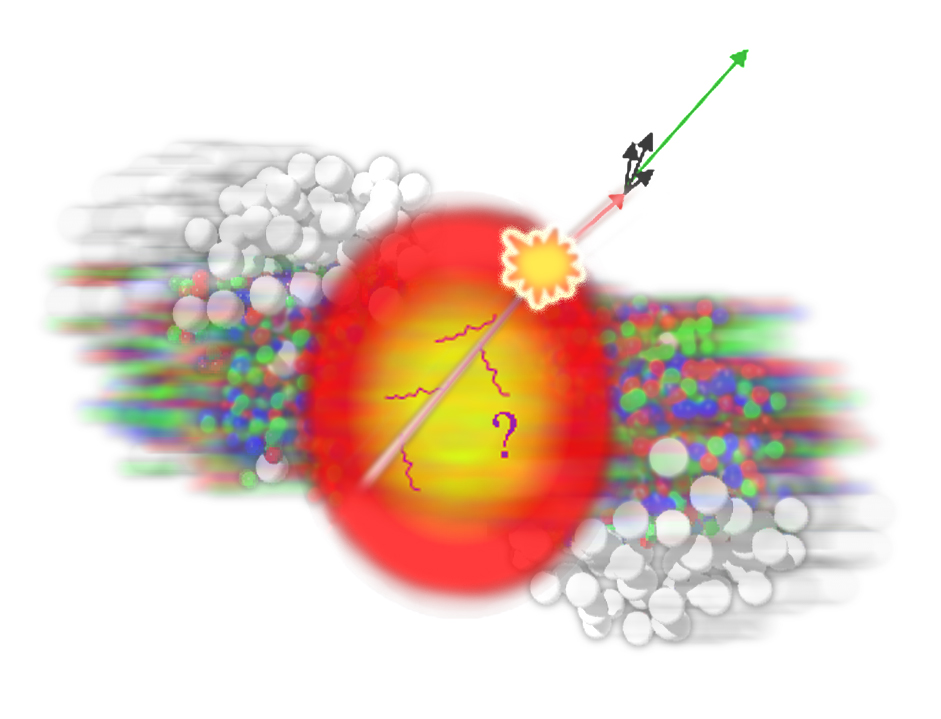
\includegraphics[width=0.5\linewidth]{jet-quenching.jpg}


%\small{Jets in a QCD medium.}
%\begin{tikzpicture}
%\node[circle,draw,inner sep=2.5cm,fill overzoom image=front] (A) {};
%\end{tikzpicture}
\end{center}


\vspace*{1cm}
\begin{minipage}{0.45\linewidth}
\begin{flushleft}   
Supervisors:\\Edmond Iancu\\Gregory Soyez\\{\bf CEA Saclay}
\end{flushleft}   
\end{minipage}
\begin{minipage}{0.45\linewidth}
\begin{flushright}
Internship\\M1 General Physics\\{\bf Paris-Sud University}
\end{flushright}
\end{minipage}

\end{titlepage}

%About 20 pages for this

\maketitle
\newpage
\pagenumbering{arabic}
\section{Introduction}


Among the many aims of the Large Hadron Collider (LHC) at CERN is the study of \emph{quark gluon plasma} (QGP), a phase of matter existing at high temperatures or densities in which quarks and gluons are deconfined. This can be compared to everyday conditions, in which quarks and gluons are confined inside hadrons. According to our models of the early universe, QGP existed for a few microseconds after Big Bang -- until the universe cooled down enough for hadronization to take place. It is re-created in high energy Pb-Pb collisions at the LHC.


The QGP created at the LHC has a very short lifetime, on the order of 10 fm ($\sim 10^{-23}$ seconds), making it difficult to study. After this time it will hadronize, and the resulting vast number of hadrons is observed experimentally. From the measured distribution of final particles, including their properties such as momentum and correlations, one then has to try to extract information about the QGP that was present at intermediate stages. 


One very useful tool is to study the propagation of energetic jets through the QGP. Here, \emph{jet} refers to a collimated spray of particles generated via successive branchings of a parton with high energy (and high virtuality) produced in the collision. When such a jet is produced in a Pb-Pb collision, it will interact with the surrounding medium (i.e. the QGP). These interactions modify the structure of the jet, for example by triggering additional branchings and thus leading to energy loss of the jet. The overall modification of the jet by the medium is known as \emph{jet quenching}. Measuring the jet quenching can give valuable information about the QGP, such as its temperature. 



In order to extract the properties of QGP out of the data from events in which jets were produced, we need a thorough theoretical understanding of how the jets interact with the medium. Thanks to asymptotic freedom in QCD, the branchings in high energy jets can be treated perturbatively -- however, there is still the need to take into account the multiple scatterings of the jet off the medium when studying the branchings. These scatterings must be resummed to all orders, a calculation that was first done about 20 years ago for a single gluon emission \cite{Baier:1996kr,Zakharov:1997uu}. In recent years the same approach has been extended to an arbitrary number of such emissions\cite{Blaizot:2012fh,Blaizot:2013hx}: an effective theory has been derived from first principles in QCD, depicting the in-medium jet evolution as a Markovian stochastic process. Among other things, this theory predicts a new mechanism for energy loss by the jet via the same type of energy cascades as are found in {\em wave turbulence}. The predictions from this new mechanism are at least qualitatively consistent with the phenomenology of jet
quenching at the LHC \cite{Aad:2010bu,Chatrchyan:2011sx}.

In the effective theory mentioned above, the successive branchings are independent from each other, making it suitable for Monte Carlo simulations. The goal of this internship is to create such a simulation, and to become familiar with the effective theory in general. While Monte Carlo simulations are already implemented in detail for jet evolution in vacuum (see \cite{Pythia,Herwig} for widely-used generic-purpose generators or \cite{SmallR} for a recent simplified implementation), there is so far no similar implementation for the in-medium case. (But see \cite{Zapp:2012ak,Schenke:2009gb} for alternative approaches.) 



The structure of this report is as follows: 
In section \ref{general} we give some general features of parton branching and jet evolution. After this, we turn our attention to the in-medium case in section \ref{medium} and describe the physics of our model, introducing the mechanism of democratic branching. In section \ref{stochastic} we give the one-dimensional stochastic model for the in-medium jet evolution and discuss some of the predictions. Then, the Monte Carlo implementation of this stochastic model is described in section \ref{simulation} and some results are shown and discussed. Finally in section \ref{perspective} the main findings are summarized and future work is briefly discussed.


\section{Parton branching and jet evolution}\label{general}

In this section we consider the evolution of a jet through parton branching, giving a brief general discussion and some considerations about the in vacuum evolution.

\subsection{Formation time}


The first important ingredient when considering the evolution of a jet is the formation time of the partons it radiates. In this section we define this formation time and estimate its value as a function of the energy of the radiated parton. 

We will assume that we are in a high energy limit, where we can neglect the masses. In this context let us consider a  1-2 parton branching, such as $g\rightarrow gg$.
For this process to be kinematically allowed, either the incoming gluon must be time-like or we must have some scattering that affects the momenta. This can be seen from the following argument: assume that we have an incoming gluon with 3-momentum $\mathbf{P}=(\mathbf{0_\perp},P_z)$ and two outgoing gluons with $\mathbf{k_1}=(\mathbf{k_\perp},xP_z)$ and $\mathbf{k_2}=(-\mathbf{k_\perp},(1-x)P_z)$:
%\begin{center}
%\begin{overpic}[width=0.4\linewidth]{branching.eps}
%\put(15,21){$P$}
%\put(90,25){$k_1$}
%\put(90,8){$k_2$}
%\end{overpic}
%\end{center}
\begin{equation}
\begin{gathered}
\begin{tikzpicture}
    \node[anchor=south west,inner sep=0] (image) at (0,0) {\includegraphics[width=0.4\textwidth]{branching.eps}};
    \begin{scope}[x={(image.south east)},y={(image.north west)}]
        \draw[] (0.70,0.35) arc (-20:20:0.5);
        \node[] at (0.15, 0.65) {$P$};
        \node[] at (0.95, 0.25) {$k_1$};
		\node[] at (0.95, 0.75) {$k_2$};
        \node[] at (0.8, 0.5) {$\theta_{12}$};
    \end{scope}
\end{tikzpicture}
\end{gathered}
\end{equation}
If the final gluons are on shell, $k_1^2=k_2^2=0$, (which they must be in the end, in order to be radiated), energy-momentum conservation gives the 4-momentum squared of the initial gluon as:
\begin{equation}
P^2=(k_1+k_2)^2=2 k_1 \cdot k_2=2(E_1E_2-\mathbf{k_1}\cdot\mathbf{k_2})=2E_1E_2(1-\cos\theta_{12}).
\end{equation}
This leads us to the conclusion that \emph{either} the initial gluon is time-like, $P^2>0$, which for the limit where we neglect the mass means off shell, \emph{or} the branching angle $\theta_{12}=0$ (meaning that the branching is strictly collinear).


The typical situation in a high energy process is to have a leading particle that is time-like, as it is produced in a hard process. We shall later consider the situation where there is scattering off a medium, which can make this 1-2 process possible even if the leading particle is on shell (since the scattering can put the initial parton off shell, or put a final off shell parton on shell again).

Regardless of whether the branching is due to virtuality or scattering, due to the uncertainty principle the branching is not instantaneous. We can define a formation time $\Delta t_f$ related to the uncertainty in the moment at which the branching took place:
\begin{equation}
\Delta t_f=\frac{1}{|E_f-E_i|}.
\end{equation}
Here the energies are the \emph{would be} energies if the partons were on shell, $E_i=E_P=\sqrt{0+P_z^2}=P_z$ and $E_f=E_{k_1}+E_{k_2}=\sqrt{{k_1}_\perp^2 + {k_1}_z^2}+\sqrt{{k_2}_\perp^2 + {k_2}_z^2}$, as seen in old fashioned perturbation theory. Noting that ${k_i}_\perp^2\ll {k_i}_z^2$ the latter can be expanded into $E_f \simeq {k_1}_z+{k_2}_z + \frac{{k_1}_\perp^2}{2{k_1}_z}+\frac{{k_2}_\perp^2}{2{k_2}_z}$. By conservation of longitudinal momentum (as seen by our notation ${k_1}_z=xP_z$, ${k_2}_z=(1-x)P_z$), and by conservation of transverse momentum ($\mathbf{k_1}_\perp+\mathbf{k_2}_\perp=\mathbf{0}\Rightarrow {k_1}_\perp={k_2}_\perp \equiv k_\perp$), we find
\begin{equation}
E_f-E_i \simeq \frac{{k_1}_\perp^2}{2{k_1}_z}+\frac{{k_2}_\perp^2}{2{k_2}_z} = \frac{k_\perp^2}{2x(1-z)P_z}.
\end{equation}
This gives us the formation time as
\begin{equation}\label{formation}
\Delta t_f \simeq \frac{2x(1-x)P_z}{k_\perp^2}\simeq \frac{2 \omega}{k_\perp^2},
\end{equation}
where the last estimate follows from noting that behaviour of the formation time mostly depends on the longitudinal momentum (or equivalently energy) of the softest of the child gluons, denoted by $\omega$. Depending on the value of $x$ we have either $\omega=xP_z$ or $\omega=(1-x)P_z$.%It is important to note the consequence of this estimate: we favour branchings in which one of the final partons is very soft, since for these branchings the formation time is shorter.

For an alternative derivation, let us consider another argument which brings more insight into the physical interpretation of the formation time. As mentioned before we define the formation time from the uncertainty in where the vertex is. We can also see it this way: before a time $\Delta t_f$ has passed, we cannot tell if an "emitted" gluon is just a virtual fluctuation that will be reabsorbed, or if it will radiate away. The criterion, in order to consider the gluon as being separated enough from its parent parton to be independent, is that the separation distance $\Delta x_\perp$ is larger than its transverse de Broglie wavelength $\lambda_\perp=1/k_\perp$. We then say that it has lost coherence with its parent. The situation is illustrated below for $q\rightarrow qg$: % in figure \ref{gluonemission}. (Or just put this inline with the text)

%\begin{figure}
\begin{equation}
%\begin{center}
\begin{gathered}
\begin{tikzpicture}
    \node[anchor=south west,inner sep=0] (image) at (0,0) {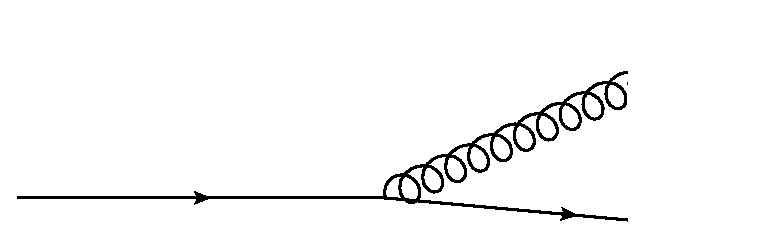
\includegraphics[width=0.5\textwidth]{gluonemission.eps}};
    \begin{scope}[x={(image.south east)},y={(image.north west)}]
        \draw[] (0.70,0.11) arc (-12:21:0.7);
        \node[] at (0.65, 0.7) {$\omega,k_\perp$};
        \node[] at (0.74, 0.27) {$\theta$};
        \draw[red,thick,dashed, <->] (0.83,0.1) -- (0.83,0.7);
        \node[red,right] at (0.83, 0.35){$\Delta x_\perp$};
        \draw[blue,thick, dashed,<->] (0.5,0) -- (0.83,00);
        \node[blue,below] at (0.65, 0){$\Delta t_f$};
    \end{scope}
\end{tikzpicture}
\end{gathered}
%\caption{Gluon losing coherence with leading particle. (Add wavelength.)}\label{gluonemission}
%\end{center}
%\end{figure}
\end{equation}

As seen in the diagram, after a time $\Delta t$ we have an angle $\theta\sim k_\perp/\omega$ related to the transverse momentum of the gluon. This leads to a separation distance that is roughly
\begin{equation}
\Delta x_\perp\sim \theta \Delta t \sim \frac{k_\perp}{\omega}\Delta t.
\end{equation}
Our criterion now turns into
\begin{equation}\label{formationk}
\lambda_\perp<\Delta x_\perp \Rightarrow \frac{1}{k_\perp}<\frac{k_\perp}{\omega}\Delta t \Rightarrow \Delta t > \frac{\omega}{k_\perp^2}.
\end{equation}
This is, up to a factor 2, what we found from the time energy uncertainty in equation \eqref{formation}. Since both lines of reasoning build on using the uncertainty (either in time or in space) this should not come as a surprise. 

\subsection{Bremsstrahlung in vacuum}
Before focussing on the in-medium evolution in the next section, we will here make a couple of observations about bremsstrahlung in vacuum. First a general statement, that holds also in medium: in QCD there are three possible parton branching processes. These are:
\begin{equation}\label{branchingdiagrams}
\begin{gathered}
\begin{overpic}[width=0.6\linewidth]{splittings.eps}
\put(3,0){$q\rightarrow qg$}
\put(38,0){$g\rightarrow \bar{q}q$}
\put(72,0){$g\rightarrow gg$}
\end{overpic}
\end{gathered}.
\end{equation}
Connected to these possibilities are the splitting functions, which can be found in e.g. \cite{peskin} as\footnote{For the splitting functions used in e.g. DGLAP there are also "loss terms" to ensure probability conservation. These are not necessary for the purpose of this discussion}
\begin{equation}\label{splittingrates}
\begin{split}
P_{q \leftarrow q}(z)&=C_F \left[ \frac{1+z^2}{1-z} \right] \\
P_{g \leftarrow q}(z)&=C_F \left[ \frac{1+(1-z)^2}{1-z} \right]\\
P_{q \leftarrow g}(z)&=\frac{1}{2} \left[ z^2+(1-z)^2\right]\\
P_{g \leftarrow g}(z)&=2 N_C \left[\frac{1-z}{z}+ \frac{z}{1-z}+z(1-z) \right],
\end{split}
\end{equation}
with $N_C=3$ and $C_F=(N_C^2-1)/(2N_C)=4/3$. These functions give the probabilities of emission of a parton from another. Consider, for example, the first kind of branching $q\rightarrow qg$. It can be seen either as an emission of a quark from a quark (with a gluon being the other emission product) or an emission of a gluon from a quark (with a quark being the other emission product). The probabilities $P_{q \leftarrow q}$ and $P_{g \leftarrow q}$ clearly complement each other in describing this situation: both have a pole for a soft $gluon$ corresponding to $z \rightarrow 1$ for the quark in $P_{q \leftarrow q}$ and $z \rightarrow 0$ for the gluon in $P_{g \leftarrow q}$. The pole for soft gluons is also found in $P_{g \leftarrow g}$ which is symmetric in $z$ and $1-z$. There is no such pole for soft $quarks$, indeed $P_{q \leftarrow g}$ has no pole at all. All this leads to the conclusion that the splitting functions strongly favour the emission of soft ($z\ll 1$) gluons. 

Note that these splitting functions are the same in the medium since they are found from the vertices in the diagrams \eqref{branchingdiagrams}. What is different from the in medium case is the angular (or transverse momentum) distribution of the radiation. For future reference let us therefore consider this spectrum for vacuum radiation. For example for $g\rightarrow gg$, the differential probability to emit a gluon with transverse momentum $\mathbf{k}_\perp$ (the bremsstrahlung spectrum) reads\cite{peskin}
\begin{equation}
\frac{\mathrm{d}P}{\mathrm{d}z\mathrm{d}^2\mathbf{k}_\perp} =\frac{{\alpha_s}}{2\pi^2}\frac{P_{g\leftarrow g}(z)}{k_\perp^2},
\end{equation}
assuming for simplicity that the parent gluon has no transverse momentum. Here $k_\perp^2$ refers to any of the child gluons' momenta squared, since they are equal. Noticing that $\frac{\mathrm{d}k_\perp^2}{k_\perp^2} = \frac{\mathrm{d}\theta^2}{\theta^2}$ we can deduce that bremsstrahlung favours collinear emission in which the child gluons propagate at small $\theta$ with respect to the parent gluon. The same conclusion holds for all elementary branchings considered in the diagrams \eqref{branchingdiagrams}. Altogether we can conclude that in vacuum, the radiation is predominately made up of \emph{soft and collinear gluons}.


\section{Medium induced jet evolution}\label{medium}
From now on we consider jets produced by a hard process inside a dense QCD medium created in a heavy ion collision. In this context the partons from the jet can scatter off partons in the medium, and as a consequence even on shell partons of the jet can radiate. For simplicity, in what follows we shall consider the situation where the leading particle is on shell. Physically, this means that we consider a leading particle that was produced long before it enters the medium at time $t=0$. 

In this section we will first discuss the properties of our medium in section \ref{themedium}, then the medium induced radiation. For the latter we focus first on a single branching in section \ref{mediuminduced} and then on multiple branchings in section \ref{multiplebranchings}

\subsection{The medium}\label{themedium}

We assume that our medium is a weakly coupled, deconfined quark gluon plasma that is in equilibrium at a temperature T. In this medium we have scattering between the partons of the jet ($\omega \gg T$) and thermal particles ($\omega \sim T$). The assumption about thermal equilibrium is a simplification, but the extension to a more general situation such as a longitudinally expanding QGP would not change the picture on a conceptual level.


Although the coupling is weak, there are effects of the gauge interaction which cannot be expanded out in perturbation theory, meaning that they must be kept in the leading order theory. One important effect of this kind is the screening of the gauge interaction by the plasma constituents, associated to the mobility of the colour charges. In analogue to what happens in an electromagnetic plasma, this leads to Debye screening. Specifically, the Coulomb potential of a charge $Q$ gets an exponential decay at large distances:
\begin{equation}
A_0(r)=\frac{Q}{r}e^{-m_Dr}.
\end{equation}
To lowest order in perturbative QED, one finds (for an ultrarelativistic plasma made of electrons, positrons and photons) $m_D\sim e^2 T^2$. Similarly, for an ultrarelativistic QCD plasma, where $A_0\rightarrow A_0^a$ and $Q\rightarrow Q^a$ refer to the colour fields and charges, one has $m_D\sim \alpha_s T^2$\cite{Debye}. The corresponding length scale is called the Debye length $\lambda_D=1/m_D$.
A Fourier transform of this potential yields
\begin{equation}
\tilde{A}_0(q)=\frac{Q}{q^2+m_D^2}.
\end{equation}
At high energy we are only interested in the screening in the transverse direction, since the Lorentz contraction leads to the interactions being controlled by the exchange of transverse momentum. Taking this into account we write instead 
\begin{equation}\label{Debye}
\tilde{A}_0(q)=\frac{Q}{q_\perp^2+m_D^2}.
\end{equation}


Together with the Debye length, it is also relevant to consider the mean free path between scatterings, which is related to the collision rate $\Gamma=v_{rel}\sigma n $ for a given relative velocity $v_{rel}$ of the test charge and a given density $n$ of the thermal quarks and gluons. We also need the total cross section $\sigma$. The differential cross section for an elastic scattering between a test charge and a constituent of the medium has a standard Rutherford form modified by the Debye screening as given in equation \eqref{Debye}:
\begin{equation}
\frac{\mathrm{d\sigma}}{\mathrm{d}^2q_\perp}\propto\frac{\alpha_s^2}{(q_\perp^2+m_D^2)^2},
\end{equation}
leading to the total cross section 
\begin{equation}
\sigma_{tot}=\int \mathrm{d}^2q_\perp\,\frac{\mathrm{d\sigma}}{\mathrm{d}^2q_\perp}=\frac{\alpha_s^2}{m_D^2}\sim\frac{\alpha_s}{T^2}.
\end{equation}
This cross section is dominated by the exchange of the softest transverse momenta, of order $m_D$, so we can see that the typical exchanged transverse momentum during interactions in the medium is $|\mathbf{q}_\perp|\sim m_D$. 



With this cross section we return to the mean free path. We consider a relativistic test charge, $v_{rel}\sim 1$. The density of the medium goes as $T^3$ and altogether we have the rate of interaction
\begin{equation}
\Gamma = v_{rel}\sigma n \sim \frac{\alpha_s}{T^2}T^3= \alpha_sT.
\end{equation}
Hence,
\begin{equation}
\lambda_{mfp}=\frac{1}{\Gamma}\sim \frac{1}{\alpha_sT}.
\end{equation}
A more careful calculation would give a logarithmic correction, but for the purpose of comparing this length scale with the Debye length this level of accuracy is enough. Recalling that $\lambda_D\sim 1/(\sqrt{\alpha_s}T)$, for a weakly coupled QGP
\begin{equation}
\lambda_{mfp}\gg\lambda_D.
\end{equation}
The Debye length $\lambda_D$ tells us over which scale interactions disappear, thereby setting the scale for possible correlations. Since the mean free path is much larger than $\lambda_D$, the scattering centres are \emph{independent} from each other. Because of this, the path of the test charge when traversing the plasma can be considered a random walk, where the transferred transverse momenta from each scattering add in quadrature. After a time $\Delta t \gg \lambda_{mfp}$ during which we have multiple independent scatterings we get (assuming no initial transverse momentum)
\begin{equation}\label{mombroad}
\langle k_\perp \rangle = 0, \quad \langle k_\perp^2 \rangle \sim \hat{q}\Delta t,
\end{equation}
where the constant of proportionality $\hat{q}$ is a transport coefficient of the medium, known as the jet quenching parameter. To get a parametric estimate of $\hat{q}$ we consider that during each scattering typically a squared momentum $m_D^2$ is gained. Hence for $\Delta t \sim \lambda_{mfp}$ we have $\langle k_\perp^2 \rangle \sim m_D$ and so
\begin{equation}
\hat{q}\sim \frac{m_D^2}{\lambda_{mfp}}=\frac{\alpha_s T^2}{1/(\alpha_s T)}=\alpha_s^2 T^3\sim m_D^2 \sigma_{tot} n,
\end{equation}
where the last estimate shows that the jet quenching parameter measures the density of the plasma constituents.


\subsection{Medium induced radiation}\label{mediuminduced}
The elastic collisions between the partons from the jet and the medium constituents are responsible not only for the transverse momentum broadening seen in equation \eqref{mombroad} but also for inducing additional radiation. As seen in equation \eqref{formationk}, a larger transverse momentum due to the scattering will reduce the formation time.

We study a jet initiated by an incoming on shell parton (the "leading particle") with a relatively high initial energy $E\gg T$. We shall use $\omega$ and $\mathbf{k}_\perp$ for the energy and transverse momentum of a generic parton in the cascade developed by the leading particle. Note that in this text \emph{cascade} and \emph{jet} are used interchangeably to refer to the cascade of partons originating from the leading particle, although in many other contexts the \emph{jet} is defined from a cone around the jet axis with a certain angle and thus excludes partons in the cascade propagating at larger angles.


The kinematics at LCH place us in the regime
\begin{equation}
\Delta t_f \sim \frac{\omega}{k_\perp^2}\gg \lambda_{mfp}\sim \frac{1}{\alpha_s T},
\end{equation}
meaning that multiple scatterings contribute coherently to a single emission:
\begin{equation}
\begin{gathered}
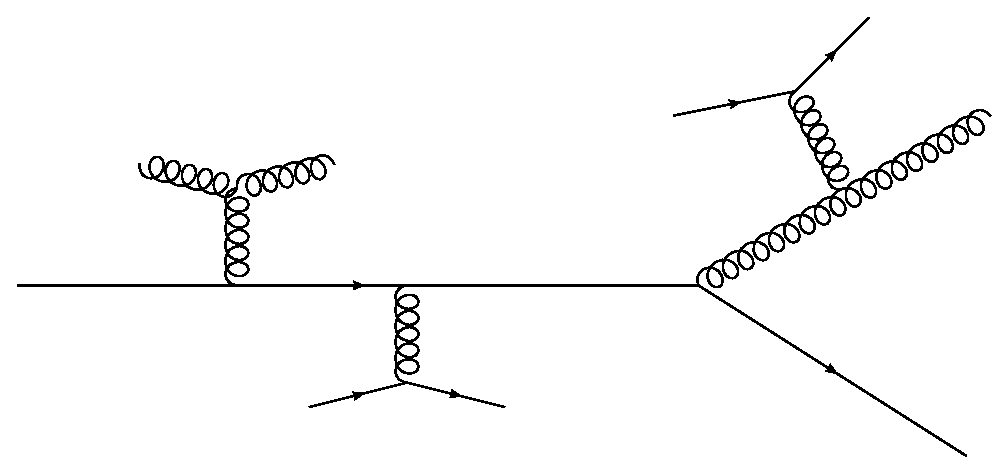
\includegraphics[width=0.5\linewidth]{scattering.eps}
\end{gathered}.
\end{equation}
As we saw in equation \eqref{formationk} the estimate of the formation time involves the transverse momentum of the gluon.
Inside the medium, the transverse momentum can be acquired by the gluon while it is about the be emitted, i.e. during the formation time itself, via rescattering. Hence, $k_\perp^2$ itself depends on $\Delta t$: $k_\perp^2|_{\Delta t_f} \equiv k_f^2 \sim \hat{q} \Delta t_f$. Thus
\begin{equation}
\Delta t_f \sim \frac{\omega}{\hat{q} \Delta t_f} \Rightarrow \Delta t_f \sim \sqrt{\frac{\omega}{\hat{q}}}.
\end{equation}
As we now see, to find the formation time it is enough to know the energy $\omega$ of the gluon since the transverse momentum can be found using the jet quenching parameter.



If we have energy scales $\omega$ and $T$ such that the formation time is much larger than the mean free path, then we are in the regime where multiple scatterings contribute coherently to a single emission. This is called the LPM ( Landau-Pomeranchuk-Migdal) regime. Of course we also need to have enough time to emit the gluon inside the medium, so the following constraints must be fulfilled for the model to be valid: $L\gg\Delta t_f(\omega)\gg \lambda_{mfp}$. Since $\Delta t_f$ is proportional to $\sqrt{\omega}$, this also gives constraints on the energy:  $\omega_c=\hat{q}L^2\gg\omega\gg T$, where the critical energy $\omega_c$ is the energy of the most energetic gluon that can be emitted through the process of multiple scattering in a medium of size $L$. 


Compared to the vacuum case, where the bremsstrahlung favoured collinear branching, now the angle $\theta_f$ at the formation time is given by
\begin{equation}
\theta_f=\frac{k_f}{\omega}=\frac{\sqrt{\hat{q}\Delta t_f}}{\omega}=\left( \frac{\hat{q}}{\omega^3} \right)^{1/4},
\end{equation}
which for a small $\omega$ is large. Since we have already concluded that the formation time is short for small $\omega$, and that the splitting functions have poles for soft gluons but not for soft quarks, we can draw the conclusion that the medium induced radiation favours \emph{soft gluons at large angles}.



We now want to compute the spectrum obtained. The differential probability to emit a gluon of energy $\omega$ via the aforemented mechanism is given by 
\begin{equation}\label{spectrum}
\frac{\mathrm{d}P}{\mathrm{d}\omega} =\frac{\bar{\alpha}}{\omega}\frac{L}{\Delta t_f(\omega)}= \bar{\alpha}\sqrt{\frac{\omega_c}{\omega^3}}.
\end{equation}
Here ${\bar{\alpha}}/{\omega}$ comes from the familiar bremsstrahlung spectrum, with $\bar{\alpha}={\alpha_s N_c}/{\pi}$. ${L}/{\Delta t_f(\omega)}$ corresponds to the temporal phase space available for an emission of a gluon with energy $\omega$ in a medium of size $L$. 

The conventional spectrum is obtained from multiplying equation \eqref{spectrum} by $\omega$. For the problem at hand this has first been computed by Baier, Dokshitzer, Mueller, Peigné, Schiff and Zakharov and is therefore called the BDMPS-Z spectrum for gluon radiation\cite{Baier:1996kr,Zakharov:1997uu}:
\begin{equation}\label{BDMPS}
\omega \frac{\mathrm{d}P}{\mathrm{d}\omega} =\bar{\alpha}\sqrt{\frac{\omega_c}{\omega}}.
\end{equation}

An important application of the above formula is the computation of the average energy lost by the leading particle:
\begin{equation}\label{average}
\Delta E = \int_T^{\omega_c} \mathrm{d}\omega \, \omega \frac{\mathrm{d}P}{\mathrm{d}\omega} \sim \bar{\alpha} \omega_c=\bar{\alpha}\hat{q}L^2.
\end{equation}
This has the following physical interpretation: the integral is dominated by the upper limit, i.e. by the most energetic gluon emissions; these emissions occur with a probability $\bar{\alpha}$, hence the energy loss goes as $\bar{\alpha}\omega_c$. However, as we shall see later, this is not the energy loss of a \emph{typical} event.
%We start by considering the bremsstrahlung spectrum, which we have already shown favours soft gluons. We can thus restrict our attention to $P_{g\leftarrow g}$. Through the multiple scattering we get the transverse momentum needed to get a branching without having to consider a time-like initial parton. We can repeat the procedure of multiple scatterings inducing a branching, but for this we must take into account that each such "cycle" takes a certain time. (add details, such as where we get $\bar{\alpha}$). Over a distance such as the size $L$ of the medium, we get $L/\Delta t_f$ times the bremsstrahlung spectrum for gluons.



\subsection{Multiple branchings in a medium}\label{multiplebranchings}

The very hard (and rare) gluon emissions with energies $\omega \sim \omega_c$, which as we have seen control the energy loss of the leading particle (see equation \eqref{average}), propagate at small angles w.r.t. the jet axis, $\theta_f(\omega_c) \sim (\hat{q}/\omega_c^3)^{1/4} \sim 1/\sqrt{\hat{q}L^3}$. Hence, they cannot contribute to the energy loss of the jet \emph{as a whole}, where here we mean the experimentally measured jet as defined by the jet opening angle $\theta_j$. One typically has $\theta_j=0.2-0.4$, which is indeed much larger than $\theta_f(\omega_c) \leq 0.1$. The experimental observation of the phenomenon of \emph{di-jet asymmetry} (a strong energy imbalance between two jets propagating back-to-back) in Pb-Pb collisions at the LHC\cite{Aad:2010bu,Chatrchyan:2011sx} demonstrates that a jet propagating through a QGP can lose a significant fraction of its energy via soft radiation ($\omega \lesssim 2$ GeV) propagating at \emph{very} large angles $\theta \gg \theta_j$. The primary gluons which are directly emitted at such large angles are too soft to carry a significant amount of energy. However, as we shall explain in what follows, energy can still be transmitted to large angles via the successive branchings of primary gluons whose energies are relatively hard, but still much smaller than $\omega_c$.


%There is one final piece needed for our puzzle: why do we not find most of the energy just outside of the cone used to define the jet? While there is some transverse momentum given to the gluon that gets radiated away from the jet, this is in general not enough to ensure that the gluon propagates with a large angle with respect to the jet axis. Since the primary gluons of interest are typically quite hard, their angles $\theta \sim k_\perp/\omega$ are still rather small.

%What we haven't considered yet, is that each radiated gluon 

The key observation is that such primary gluons will \emph{keep branching}. During this branching they will decay into a large number of very soft gluons, but since the formation time is dependent on the energy it also becomes possible to have branchings in which the energy is split fairly evenly between the child gluons. Such branchings are called democratic branchings and provide a very efficient mechanism for transfer of energy down to soft scales and large angles. Indeed, we can envisage an energy cascade, which is something that is more familiar in the context of wave turbulence. This will be seen in more detail in section \ref{stochastic}.



To understand why multiple branching will occur, let us return to the differential probability for a single emission in equation \eqref{spectrum}. The total probability to emit a gluon with energy $\omega>\omega_0$ for a given soft scale $\omega_0$ is obtained as
\begin{equation}\label{omega0}
P(\omega>\omega_0)=\int_{\omega_0}^\omega \mathrm{d\omega'}\, \frac{\mathrm{d}P}{\mathrm{d}\omega'} \sim \bar{\alpha}\sqrt{\frac{\omega_c}{\omega_0}} = \bar{\alpha}\sqrt{\frac{\hat{q}}{\omega_0}}L.
\end{equation}
The integration is now dominated by the \emph{lower} limit, so equation \eqref{omega0} is in essence the probability to emit a gluon with energy $\omega_0$. (The fact that this diverges for $\omega_0 \rightarrow 0$ demonstrates the tendency of the medium induced gluon cascade to emit very soft gluons.) The expression above is well defined as a probability as long as it remains smaller than 1. When this quantity becomes of $\mathcal{O}(1)$, it is a signal that we need to consider multiple branchings. From equation \eqref{omega0} this happens when $\omega_0$ is soft enough: 
\begin{equation}\label{omegabr}
\omega_0 \lesssim \omega_{br} \equiv \bar{\alpha}^2\omega_c=\bar{\alpha}^2 \hat{q} L^2.
\end{equation}
This $\omega_{br}$ is the energy scale for the onset of multiple branchings in the medium induced gluon cascade. More precisely, equation \eqref{omegabr} suggests that gluons with $\omega \sim \omega_{br}$ are emitted with a probability of $\mathcal{O}(1)$ (meaning that there is a number of $\mathcal{O}(1)$ of such gluons in a typical event). Gluons which are even softer ($\omega \ll \omega_{br}$) will be produced in great numbers in each event -- however, such very soft gluons carry little energy. As we shall see, the energy loss by the jet is ultimately controlled by primary gluon emissions with $\omega \sim \omega_{br}$.



In the above discussion we implicitly assumed that the scale $\omega_{br}$ is smaller than the energy $E$ of the leading particle. This is indeed the case in the kinematical regime for jets in heavy ion collisions at the LHC, where $E\gtrsim $ 100 GeV while a typical value for $\omega_{br}$ is 5-10 GeV. (This corresponds to $\hat{q} \sim$ 1-2 $\text{GeV}^2/\text{fm}$ and a medium size of $L\sim$ 4 fm.)\cite{Review}

The fact that $E\gg \omega_{br}$ implies that the leading particle can emit a large number of soft ($\omega \leq \omega_{br}$) gluons without losing a considerable amount of energy. In fact one can anticipate from the discussion above (and it will later be confirmed through calculations) that the energy lost by the leading particle in a \emph{typical} event must be of $\mathcal{O}(\omega_{br})$.


Equation \eqref{omega0} can also be used to estimate the typical separation in time between two successive soft branchings. When $\omega_0 \ll \omega_{br}$ the probability $P(\omega>\omega_0)$ becomes of $\mathcal{O}(1)$ already for times $ \Delta t < L$, namely for $\Delta t\sim \Delta t_{br}$ with
\begin{equation}
\Delta t_{br}(\omega_0)=\frac{1}{\bar{\alpha}} \sqrt{\frac{\omega_0}{\hat{q}}} = \frac{1}{\bar{\alpha}} \Delta t_f(\omega_0).
\end{equation}
Here, we can see that the time between two successive branchings is parametrically larger than the formation time for a single emission. This is a necessary condition for successive branchings to be viewed as independent from each other. 

So far we have the picture for a typical event where the leading particle emits a number of $\mathcal{O}(1)$ of gluons with energy $\omega_{br}$ together with a large number of softer gluons. The question is what happens to these primary gluons after being emitted. We would like to argue that they in turn generate gluon cascades via multiple branchings and that the energy flow along this cascade is controlled by quasi-democratic branchings (emissions where the energy fraction of the two child gluons are comparable)\cite{Blaizot:2013hx}.  To this aim, let us apply equation \eqref{omega0} to a mini-jet generated by the primary gluon with initial energy $\omega$ and express $\omega_0$ as $\omega_0=z\omega$, with $z$ the energy fraction taken by the softest child gluon in the mini-jet. Then, $\Delta P = \bar{\alpha} \sqrt{{\hat{q}}/{(z \omega)}}\Delta t$ becomes of $\mathcal{O}(1)$ whenever $\Delta t \sim \Delta t_{br}(\omega)=({1}/{\bar{\alpha}}) \sqrt{{\omega}/{\hat{q}}}$ irrespective of the value of $z$, in particular also for democratic branchings with $z \sim 1-z \sim \frac{1}{2}$. Such democratic branchings are the most efficient ones when it comes to redistributing the energy of the primary gluon to its descendants. As a result, the whole initial energy $\omega$ will get degraded into a myriad of very soft ($\omega \sim T$) gluons after a time of $\mathcal{O}(\Delta t_{br}(\omega))$. In other words, the lifetime of a minijet as a whole is of the same order as the time it takes for the primary gluon to undergo the first democratic branching.
Taking all this into consideration, we arrive at the picture of a typical event shown in figure \ref{democraticbranch}.


\begin{figure}
\begin{center}
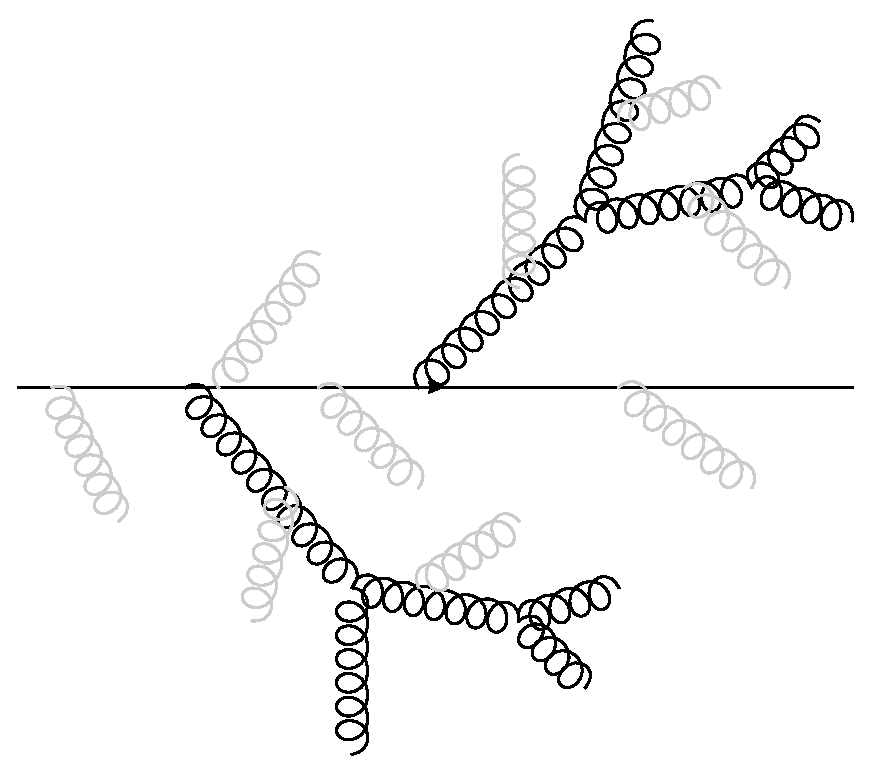
\includegraphics[width=0.5\linewidth]{democraticbranch.eps}
\end{center}
\vspace*{-20pt}
\caption{Typical event with multiple branching, where a number of $\mathcal{O}(1)$ of primary gluons are emitted from the leading particle and these primary gluons consequently branch democratically. The grey gluon lines represent the large number of non democratic, soft emissions.}\label{democraticbranch}
\end{figure}



Since as we have argued above the multiple branchings are independent, the process is Markovian. To deal with this process it is convenient to turn equation \eqref{spectrum} into a rate for gluon emission in the medium -- for a first approximation it suffices to divide the expression by the medium size $L$ to obtain
\begin{equation}\label{rate}
\frac{\mathrm{d}^2P}{\mathrm{d}\omega \mathrm{d}t} \sim \frac{\bar{\alpha}}{\omega}\frac{1}{\Delta t_f(\omega)} = \frac{1}{\omega}\frac{1}{\Delta t_{br}(\omega)}.
\end{equation}
Not surprisingly, the rate is inversely proportional to the time between two successive emissions. 



\section{Medium induced branching as a Markovian process}\label{stochastic}
In this section we describe the mathematical structure of the Markovian branching process introduced in the previous section, and summarize some of the known analytical results.
%Structure: describe model, describe what kernel we get (or, probably, discuss kernel already in previous section), then introduce probability evolution equation, moment generating functional, etc. Predictions of models, i.e. energy ending up in condensate (formally, in practice T will give lower energy scale rather than zero...). Turbulence. 

%Things to check against numerics would involve
%\begin{itemize}
%\item One point function
%\item Two point function
%\item Flow
%\item Probabilities? (First few)
%\end{itemize}
%Numerics should also check cutoff convergence. (For the things we expect to converge, so not eg number density.) Need to mention the need for this cutoff and discuss IR divergences...

\subsection{The general structure of the stochastic model}

As described by the previous section, we can formulate a one dimensional stochastic model to describe the jet quenching, see e.g. ref \cite{probabilistic}. Here, one dimensional refers to dimensions apart from the time dimension, in this case energy fractions. We will start by writing equation \eqref{rate} in a more precise way, which takes into account the energy conservation at the emission vertex. We then get the differential probability per unit time and per unit $z$ for the parent gluon with energy $\omega = xE$ to split into a pair of child gluons with energies $z\omega$ and $(1-z)\omega$ as in ref \cite{FisterIancu}:
\begin{equation}\label{preciserate}
\frac{\mathrm{d}^2 P(z,t)}{\mathrm{d}z\mathrm{d}t}=\frac{\alpha_s}{2 \pi}\frac{P_{g\leftarrow g}(z)}{\Delta t_{br}(z,\omega)},
\end{equation}
with
\begin{equation}
\Delta t_{br}(z,\omega)=\sqrt{\frac{z(1-z)\omega}{\hat{q}_{eff}(z)}}, \quad \hat{q}_{eff}(z) \equiv \hat{q}[1-z(1-z)].
\end{equation}
The branching time is a more precise version of what we have used before, and includes the effective jet quenching parameter $\hat{q}_{eff}(z)$. Note that in equation \eqref{rate} $\omega$ referred to the energy of the softest of the child gluons, while in equation \eqref{preciserate} $\omega$ refers to the energy of the parent gluon.

Equation \eqref{preciserate} shows that a natural time scale is the branching time. In order to work with dimensionless variables we use the branching time of the leading particle to define $\tau \equiv t/\Delta t_{br}(E)$. Using this definition and the splitting rate $P_{g \leftarrow g}(z)$ in equation \eqref{splittingrates}, we can rewrite equation \eqref{preciserate} as
\begin{equation}\label{ratewithkernel}
\frac{\mathrm{d}^2 P(z,\tau)}{\mathrm{d}z\mathrm{d}\tau}(z,\tau)=\frac{K(z)}{2 \sqrt{x}} \equiv K(x,z),
\end{equation}
where we for convenience have introduced the splitting kernel
\begin{equation}\label{kernel}
K(z)=\frac{[1-z(1-z)]^{5/2}}{[z(1-z)]^{3/2}}.
\end{equation}
To be able to obtain analytic results, we also consider a simple version of the kernel, in which the numerator is replaced by one. This simplified kernel is expected to behave in a similar way as the full kernel, notably it has the same poles.

With our new found splitting rate, we can consider the probability density ${P_n(\{x\},\tau)}=P_n(x_1,x_2,...x_n,\tau)$ to find $n$ gluons with energy fractions $x_i$ compared to the leading parton. This probability density will change as
\begin{equation}\label{Pevo}
\party{P_n(\{x\},\tau)}{\tau}=gain-loss.
\end{equation}
\begin{itemize}
\item Gain term: any gluon with energy fraction $x'_i$ in $P_{n-1}$ splitting as $x'_i \rightarrow z x'_i + (1-z)x'_i$, with the first of the child particles matching the energy fraction $x_i$ in $P_n$ and the second matching $x_n$ in $P_n$. This leads to a gain term 
\begin{equation}
%FIXME: limits for integrals 
gain=\sum_{i=1}^{n-1} \int \mathrm{d}x'_i \int \mathrm{d}z\, K(z,x'_i) P_{n-1}(x_1...x'_i...x_{n-1}) \delta(zx'_i-x_i)\delta((1-z)x'_i-x_n)
\end{equation}
\item Loss term: any of the gluons in $P_n(\{x\})$ branching. This leads to a loss term
\begin{equation}
%FIXME: limits for integrals 
loss=\sum_{i=1}^n \int \mathrm{d}z\, K(z,x_i) P_n(\{x\}).
\end{equation}
\end{itemize} 


Once we have our probability densities, we can use them to find expectation values for physical observables. We define the expectation value for any observable $O$ as
\begin{equation}
\langle O \rangle = \sum_{n=1}^\infty \int \mathrm{d}x_1...\mathrm{d}x_n \, P_n(\{x\},\tau) O_n(\{x\})
\end{equation}
and get the time evolution 
\begin{equation}
\party{\langle O \rangle}{\tau}=\sum_{n=1}^\infty \int \mathrm{d}x_1...\mathrm{d}x_n \, \party{P_n(\{x\},\tau)}{\tau} O_n(\{x\}).
\end{equation}
%
After insertion of the evolution equation for probability densities (equation \eqref{Pevo}) and renaming of summation indices, this turns into
%
\begin{equation}
\party{\langle O \rangle}{\tau}=\sum_{n=1}^\infty \int \mathrm{d}x_1...\mathrm{d}x_n\, P_n(\{x\},\tau) \sum_{i=1}^n \int \mathrm{d}z\, K(z,x_i) \Delta O_{n,i}(\{x\},z),
\end{equation}
with
\begin{equation}
\Delta O_{n,i}(\{x\},z)=O_{n+1}(...zx_i...(1-z)x_i)-O_n(\{x\}).
\end{equation}


It is helpful to introduce the moment generating functional $Z$, which will help us find some useful expectation values:
\begin{equation}
Z(u(x),\tau)=\sum_{n=1}^\infty \int \mathrm{d}x_1...\mathrm{d}x_n\, P_n(\{x\},\tau) u(x_1)...u(x_n).
\end{equation}
We can see $Z$ as an expectation value itself, corresponding to taking $O_n(\{x_i\}=u(x_1)...u(x_n)$. Using the general evolution equation found above, we get
\begin{multline}\label{Zevo}
\party{Z}{\tau}=\sum_{n=1}^\infty \int \mathrm{d}x_1...\mathrm{d}x_n\, P_n(\{x\},\tau)\\
 \sum_{i=1}^n \int \mathrm{d}z\, [ K(z,x_i)
u(x_1)...u(zx_i)...u(x_n)u((1-z)x_i) 
- u(x_1)...u(x_n) ].
\end{multline}
A neat way to write this is to use the functional derivative $\frac{\delta Z(u(x),\tau)}{\delta u(x)}$ with $\frac{\delta u(x_i)}{\delta u(x_j)}=\delta(x_i-x_j)$, equation \eqref{Zevo} then takes the form
\begin{equation}
\party{Z}{\tau}=\int \mathrm{d}z \int \mathrm{d}x \, K(z,x) [u(zx)u((1-z)x) - u(x)]\frac{\delta Z(u(x),\tau)}{\delta u(x)}.
\end{equation}

The above equation can now be used to find the evolution equation for the number density in $x$-space,  $n(x)=\langle \hat{n} (x)\rangle$ and the number density of pairs $n^{(2)}(x,x') = \langle \hat{n}^{(2)}(x,x') \rangle $. We define 
\begin{equation}
\hat{n}(x)=\sum_{i=1}^n \delta(x_i-x), \quad \hat{n}^{(2)}(x,x')=\sum_{i \neq j} \delta(x_i-x)\delta(x_j-x').
\end{equation}
The higher multiplicities are defined similarly. Taking these definitions together with the definition of $Z$ we find
\begin{equation}\label{moments}
n^{(k)}(x_1,x_2...x_k)=\frac{\delta Z(u(x),\tau)}{\delta u(x_1)\delta u(x_2)...\delta u(x_k)}\Bigg|_{u=1}.
\end{equation}

Physically, it is of more interest to look at energy density rather than number density, i.e. to look at the one-point function $D(x,\tau)\equiv xn(x,\tau)$ and the two-point function $D^{(2)}(x,x'\tau)\equiv xx'n^{(2)}(x,x',\tau)$, since these measure the energy distribution. Using equation \eqref{moments} we get
\begin{equation}
D(x,\tau)=x \frac{\delta Z(u(x),\tau)}{\delta u(x)}\Bigg|_{u=1},\quad D^{(2)}(x,x',\tau)=xx' \frac{\delta Z(u(x),\tau)}{\delta u(x)\delta u(x')}\Bigg|_{u=1},
\end{equation}
and after some rewriting we obtain
\begin{equation}\label{Devo}
\party{}{\tau}D(x,\tau)=\int \mathrm{d}z\, K(z) \left[\sqrt{\frac{z}{x}} D\left(\frac{x}{z},\tau\right)- \frac{z}{\sqrt{x}}D(x,\tau)  \right]
\end{equation}
and
\begin{multline}\label{D2evo}
\party{}{\tau}D^{(2)}(x,x',\tau)=\int \mathrm{d}z\, K(z) \left[ \sqrt{\frac{z}{x}} D^{(2)}\left(\frac{x}{z},x',\tau\right) - \frac{z}{\sqrt{x}} D^{(2)}(x,x',\tau)\right]+(x \leftrightarrow x') \\
+ \frac{xx'}{(x+x')^2} K\left(\frac{x}{x+x'}\right) \frac{1}{\sqrt{x+x'}} D(x+x',\tau).
\end{multline}
The rest of this section will focus on the solutions to equations \eqref{Devo} and \eqref{D2evo}, and the interpretations and consequences of these solutions.

\subsection{The gluon spectrum}\label{onepoint}
For the simplified kernel, a solution to \eqref{Devo} has been found from a Mellin transform to be\cite{Blaizot:2013hx}
\begin{equation}\label{Mellin}
D(x,\tau) = \frac{\tau}{\sqrt{x}(1-x)^{3/2}}\exp\left(-\frac{\pi \tau^2}{1-x}\right).
\end{equation}
This solution is plotted for various values of $\tau$ in figure \ref{Dfig}, and is replotted in section \ref{simulation}, figure \ref{Dtimes} together with the numerical results.




\begin{figure}
  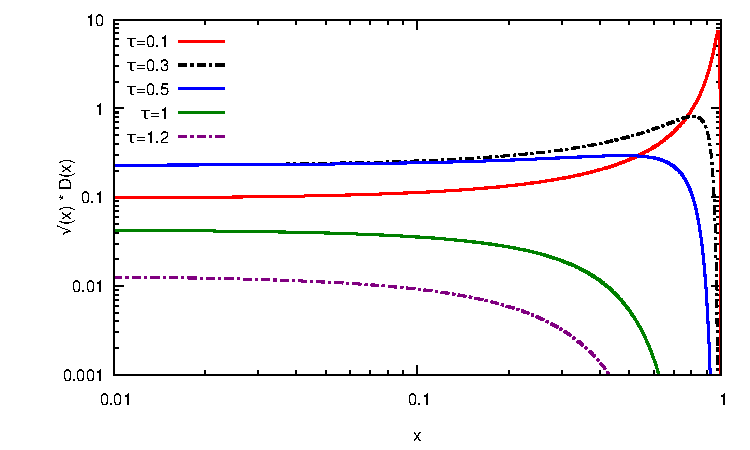
\includegraphics[width=0.9\linewidth]{plotD.pdf}
  \vspace*{-20pt}
  \caption{Plot of $\sqrt{x}D(x,\tau)$, with $D(x,\tau)$ given by equation \eqref{Mellin}, for various times $\tau$.}\label{Dfig}
\end{figure}




As seen in the figure, and also from the above equation, the spectrum has a power law tail at small $x$, namely
\begin{equation}\label{softD}
D(x,\tau)\simeq \frac{\tau}{\sqrt{x}}e^{-\pi\tau^2}.
\end{equation}
This is exactly the same behaviour for the soft $x$ dependence as in the BDMPS-Z spectrum in equation \ref{BDMPS}; in this equation $\omega=xE$, so the $1/\sqrt{\omega}$ dependence corresponds to $1/\sqrt{x}$. The fact that the spectrum at small values of $x$ is the same for a single gluon emission as for the case of multiple branchings is remarkable: apparently the fact that multiple branchings take place does not modify the spectrum. From a mathematical perspective, the evolution equation for the gluon spectrum (see equation \eqref{Devo}) has a fix point at $1/\sqrt{x}$: inserting $D_{fix}(x,\tau)=1/\sqrt{x}$ into the evolution equation would lead to a cancellation between the gain term and the loss term\cite{FisterIancu}. 
Such a fix point is known as a Kolmogorov-Zakharov fixed point in the theory of wave turbulence, and is a necessary condition for the energy flux associated with the multiple branching to be $x$-independent. (See ref \cite{FisterIancu} for further discussion of the energy flow through the spectrum.) This $x$-independence means that during the branching process, energy will be transported to softer and softer gluons without accumulating at any specific value of $x$; we have a so called turbulent energy cascade. To understand the physics behind this we must return to section \ref{multiplebranchings}, where we found that the scattering in the medium makes democratic branchings possible. The democratic branchings are efficient at transporting energy down the energy cascade and will in fact ultimately transport it \emph{out of} the cascade. The comparison between democratic gluon branching and the case of wave turbulence is illustrated in figure \ref{turbulence}.



To see what we mean by saying that energy is transported out of the cascade, we should first calculate the total energy found \emph{in} the cascade. Through a change of variables, $u=x/(1-x)$, we can integrate over all values of $x$ in equation \eqref{Mellin} to find the total energy fraction in the cascade as
\begin{equation}\label{X}
\langle X(\tau)\rangle=\int_0^1 \mathrm{d}x\, D(x,\tau) = e^{-\pi\tau^2}.
\end{equation}
We note that this energy is decreasing in time. The remaining part, $\langle \epsilon (\tau) \rangle = 1- \langle X(\tau)\rangle$, formally ends up in a condensate at $x=0$. Physically, as soon as we reach an energy scale comparable to the temperature $T$ of the QGP we expect thermalization to take place.

For small values of $\tau$, the energy loss of the cascade is given by
\begin{equation}\label{epsilon}
 \langle \epsilon(\tau) \rangle \equiv 1- \langle X(\tau)\rangle \simeq \pi \tau^2.
\end{equation}
This quantity will in the next section be compared to the \emph{fluctuations} in the energy loss at small $\tau$. To express this energy loss in physical units, recall the definition for $\tau$ (found above equation \eqref{ratewithkernel}) and the definition for $\omega_{br}$ (given in equation\eqref{omegabr}). Using these definitions for the time when the jet has travelled all the plasma, $t=L$, we get $\tau^2(L)=L^2/\Delta t^2_{br}(E)=\omega_{br}(L)/E$ and hence 
\begin{equation}
\mathcal{E}(L)=E\langle \epsilon(L) \rangle = E \left[ 1-e^{-\pi {\omega_{br}(L)}/{E}} \right] \simeq \pi \omega_{br}(L),
\end{equation}
where the last estimate holds whenever $L\ll \Delta t_{br}(E)$ or equivalently $\omega_{br}(L) \ll E$. As we predicted in section \ref{multiplebranchings} the typical energy loss is indeed of $\mathcal{O}(\omega_{br})$.


The flow of energy out of the cascade is also visible in figure \ref{Dfig}, where for the larger values of $\tau$ each subsequent curve is below the previous one. Apart from this, one can also notice the peak close to $x=1$ for small times $\tau$; this peak corresponds to the leading particle and gets washed out when $\tau$ gets close to one. Recalling that $\tau=1 \Leftrightarrow t=\Delta t_{br}(E)$, this means that for $\tau \sim 1$ the leading particle has had the time to undergo a democratic branching and is therefore no longer visible.

%(Discuss a bit more about using a cutoff $x_0$ and also about angles, make connection to what is observed... Should mention somewhere what is observed, i.e. the di-jet asymmetry and the fact that energy is recovered at large angles.)


As a final note on the one-point function: had we instead tried to compute the total \emph{number} of gluons, we would have faced an infrared divergence. Since there will be infinitely many gluons of infinitesimal energies, the total number of gluons is not a meaningful observable.



\begin{figure}
\minipage{0.5\textwidth}
	\begin{overpic}[width=\linewidth]{democratic.eps}
	\put(5,40){$x=1$}
	\put(43,47){$x \sim \frac{1}{2}$}
	\put(53,58){$x \sim \frac{1}{4}$}
	\put(68,59){\vector(4,0){8}}
	\put(64,70){$x \sim \frac{1}{8}$}
	\put(79,71){\vector(4,0){8}}
	\end{overpic}
  	%\vspace*{-30pt}
  	%\caption{here go gluons}\label{fig:D0_t1}
\endminipage\hfill
\minipage{0.5\textwidth}
  	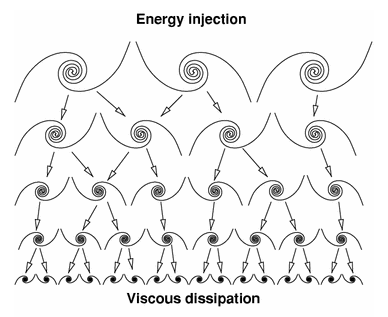
\includegraphics[width=\linewidth]{Richardson_cascade.png}
  	%\vspace*{-30pt}
  	%\caption{Turbulence}\label{fig:D0_t5}
\endminipage\hfill
\caption{Two examples of an energy cascade. To the left democratic branching of gluons, to the right wave turbulence. In both cases there is an injection of energy (for the gluons, this comes from the leading particle) followed by an efficient transport of the energy from the highest energy scale to the lowest, followed by dissipation of the energy (for the gluons, thermalization when $\omega \sim T$). Not shown here is the multitude of softer branchings in the gluon mini-jet.}\label{turbulence}
\end{figure}


\subsection{The gluon pair correlations}
The gluon spectrum given by equation \eqref{Mellin} can, in turn, be used to find the gluon pair correlations $D^{(2)}(x,x',\tau)$. By comparing \eqref{D2evo} to \eqref{Devo} it is clear that, apart from the source term, the general structure is the same. (Note however that without the source term, equation \eqref{D2evo} would give that the number of pairs is always zero if we take the initial condition of having only one single gluon and no pairs.) To see how we can exploit this structural similarity, let $L$ be an operator defined from rewriting \eqref{D2evo} as
\begin{equation}\label{Greenproblem}
\party{}{\tau}D^{(2)}(x,x',\tau) = (L_x + L_{x'})D^{(2)}(x,x',\tau)+S(x,x',\tau).
\end{equation}
Assume that we have a Green's function that is the solution to
\begin{equation}\label{Greenfunction}
\left(\party{}{\tau}- L_x\right)G(x,x_0,\tau)=0
\end{equation}
fulfilling the initial condition $G(x,x_0,\tau=0)=\delta(x-x_0)$. The solution to our problem \eqref{Greenproblem} is then given by the convolution
\begin{equation}
\int_0^\tau \mathrm{d}\tau' \int_x^1 \mathrm{d}x_1 \int_{x'}^{1-x_1} \mathrm{d}x_2\, G(x,x_1,\tau-\tau') G(x',x_2,\tau-\tau') S(x_1,x_2,\tau').
\end{equation}


What we need, then, is to find the appropriate Green's function $G(x,x_0,\tau=0)$. We can note that equation \eqref{Greenfunction} is a slight generalization of the evolution equation for the one point function $D(x,\tau)$, equation \eqref{Devo}, with a different initial condition. Our Green's function can thus be found in terms of $D(x,\tau)$ as follows (see appendix \ref{Greendetails} for details):
\begin{equation}
G(x,x_0,\tau) = \frac{1}{x_0} D\left(\frac{x}{x_0},\frac{\tau}{\sqrt{x_0}}\right),
\end{equation}
and our two-point function is given by 
\begin{equation}\label{D2}
\int_0^\tau \mathrm{d}\tau' \int_x^1 \mathrm{d}x_1 \int_{x'}^{1-x_1} \mathrm{d}x_2\, 
\frac{1}{x_1} D\left(\frac{x}{x_1},\frac{\tau-\tau'}{\sqrt{x_1}}\right)
\frac{1}{x_2} D\left(\frac{x'}{x_2},\frac{\tau-\tau'}{\sqrt{x_2}}\right)
S(x_1,x_2,\tau'),
\end{equation}
where we have taken the appropriate limits for the integrals over $x_1$ and $x_2$. The physical interpretation of this solution is as follows: in order to have a pair of gluons with energy fractions $x$ and $x'$ at time $\tau$, a new pair with $x_1$ and $x_2$ can be created at any intermediate time $\tau'$, after which they evolve separately until they have the energy fractions $x$ and $x'$ in the end. 



Evaluating the integrals in equation \eqref{D2} yields (see appendix B in ref \cite{Escobedo:2016jbm})
\begin{equation}\label{D2solution}
D^{(2)}(x,x',\tau)=\frac{1}{2\pi}\frac{1}{\sqrt{xx'(1-x-x')}}\left[ \exp\left({-\frac{\pi \tau^2}{1-x-x'}}\right) -\exp\left({-\frac{4 \pi \tau^2}{1-x-x'}}\right) \right].
\end{equation}
Through similar considerations the equations can be found for all n-point functions (which are in general also called correlations), see ref \cite{KNO}. The above solution is plotted in section \ref{simulation}, figure \ref{D2times} together with the numerical results, for $x=x'$ at various values of $\tau$. Note that at small $x$ and $x'$, $D^{(2)}(x,x')$ goes as $1/\sqrt{xx'}$. 


We can use the pair correlations to find the fluctuations in energy loss:
\begin{equation}
\sigma_\epsilon^2(\tau)=\sigma_X^2(\tau) = \langle X^2(\tau) \rangle - \langle X(\tau)\rangle ^2 ,
\end{equation}
with $\langle X(\tau)\rangle$ given by equation \eqref{X} and $\langle X^2 (\tau)\rangle$ given by
\begin{equation}
\langle X^2(\tau) \rangle =\int_0^1 \mathrm{d}x \int_0^1 \mathrm{d}x'\, D^{(2)}(x,x',\tau)+\int_0^1 \mathrm{d}x\, x D(x).
\end{equation}
Evaluation of the above expression can be found in e.g. ref \cite{Escobedo:2016jbm} to give 
\begin{equation}
\sigma_\epsilon^2(\tau) = \frac{1}{3}\pi^2\tau^4 - \frac{11}{15}\pi^3 \tau^6 + \mathcal{O}(\tau^8).
\end{equation}
By comparison with equation \eqref{epsilon}, to order $\tau^4$ we find that $\sigma_\epsilon(\tau)\simeq \langle \epsilon(\tau)\rangle/\sqrt{3}$. That is, the fluctuations in the energy loss are \emph{of the same order} as the energy loss itself! This means that the di-jet asymmetry for a given event might not be due to one jet traversing a larger distance in the medium compared to the other, but could just as well be due to the inherent fluctuations in the energy loss by the mechanism of multiple branching. 


Physically, the fact that the fluctuations are of the same order as the energy loss itself is due to the fact that both these quantities are governed by the emission of primary gluons. The number of primary gluons is of $\mathcal{O}(1)$, hence the fluctuations in the number of primary gluons must also be of $\mathcal{O}(1)$. Once a primary gluon is emitted its energy gets transported out of the cascade by the means of democratic branchings, so the number of primary gluons will be roughly proportional to the energy loss while the fluctuations in the number of primary gluons will be roughly proportional to the fluctuations in the energy loss.


Note that the above reasoning holds for small values of $\tau$. For large values of $\tau$ the fluctuations will go away, since more and more energy will end up in the condensate. As previously discussed, the regime at the LHC makes the small $\tau$ limit the one of interest.


\section{Simulation}\label{simulation}
In this section we present the implementation of a Monte Carlo simulation, and some numerical results obtained from it. The simulation treats gluons only for simplicity, which is motivated by the finding in section \ref{mediuminduced} that the in-medium radiation favours gluons. We use both the full kernel, as given in equation \eqref{kernel}, and the simplified kernel in which the numerator is replaced by one. 



%The classes created for this simulation are {\tt Particle}, {\tt Event}, {\tt GeneratorInMedium} and {\tt GeneratorInMediumSimple}. (For each describe the relevant class members. Or perhaps skip this part, doesn't tell the reader that much... focus on results.)





At the core of the simulation is a function, {\tt \char`_branch()}, that starts with an initial particle, branches it recursively during a given time and keeps track of the intermediate and final particles. For each particle in the branching a splitting time $t$ and an energy fraction $z$ is generated randomly, with a probability density function found from the splitting kernel. For the simple kernel the primitive function can be inverted both for $t$ and $z$, but in order to generate the random values of $t$ and $z$ for the full kernel the veto algorithm is used.
The pseudo code given in algorithm \ref{branchingAlg} gives the general idea of the function {\tt \char`_branch()}, with several bookkeeping variables omitted to increase readability. The code is given in appendix \ref{code} for comparison.


One important feature in the simulation that we did not have to worry about in the stochastic model up until now is the need for an infra-red cutoff. Indeed, we mentioned by the end of section \ref{onepoint} the number of gluons is not a meaningful observable. Nevertheless, a number of gluons is exactly what our simulation will produce, and unless we introduce a cutoff our function {\tt \char`_branch()} will find very soft gluons with a very short splitting time at each step. We therefore chose a cutoff $\epsilon$ well below the energy scales we are interested in, restrict our splitting kernel to values above this cutoff and stop the branching whenever the energy fractions of our gluons get too small.

%The most important function is {\tt \char`_branch()}. The pseudo code shown in algorithm \ref{branchingAlg} gives the general idea of the function, with several bookkeeping variables omitted to increase readability. This function is responsible for recursively branching the leading particle during a given branching time. The full code is given in Appendix \ref{code} for comparison. 
%The simulation is written in C++ and makes use of the GNU Scientific Library\footnote{\url{https://www.gnu.org/software/gsl/}} for generating (pseudo-)random numbers.


During the branching, each particle (including the intermediate ones) is given an index. To allow for a full reconstruction of the event, this index refers to an element in a vector. Each element is of the class {\tt Particle} which stores the following information about each particle:
\begin{itemize}
\item The index of the parent of the particle. (Set to $-1$ for the leading particle.)
\item The start time. (Set to $0$ for the leading particle.)
\item The end time. (Set to $-1$ for the particles that have not had time to branch, i.e. the final particles.)
\item The indices of the two child particles. (Set to $-1$ for the particles that have not had time to branch, i.e. the final particles.)
\item The energy fraction $x$ as compared to the leading particle. (Set to $1$ for the leading particle.)
\end{itemize}
This vector is stored in a class {\tt Event}. However, the only physical observables will be the final particles and their energy fraction. Therefore, {\tt Event} also stores a vector with only the $x$-values of the final particles. 


\begin{algorithm}
\caption{Recursive branching}\label{branchingAlg}
\begin{tt}
\begin{algorithmic}[0]
\Function{\char`_branch}{}
\State x $\gets$ parent's energy fraction
\If {x $<$ x$_{min}$} \Comment{Lower limit for x is reached}
\State \textbf{return}
\EndIf
\State t $\gets$ randomly generated time
\State z $\gets$ randomly generated energy fraction
\State time\char`_left $\gets$ total branching time minus parent's start time
\If {t $<$ time\char`_left} \Comment{No time left for branching}
\State \textbf{return}
\EndIf
\State particle\char`_vector $\gets$ particle\char`_vector + new particle
\State \char`_branch()
\State particle\char`_vector $\gets$ particle\char`_vector + new particle
\State \char`_branch()
\State \textbf{return}
\EndFunction
\end{algorithmic}
\end{tt}
\end{algorithm}





%Pileup: see figure \ref{fig:D-5}

%\begin{figure}
%\centering
%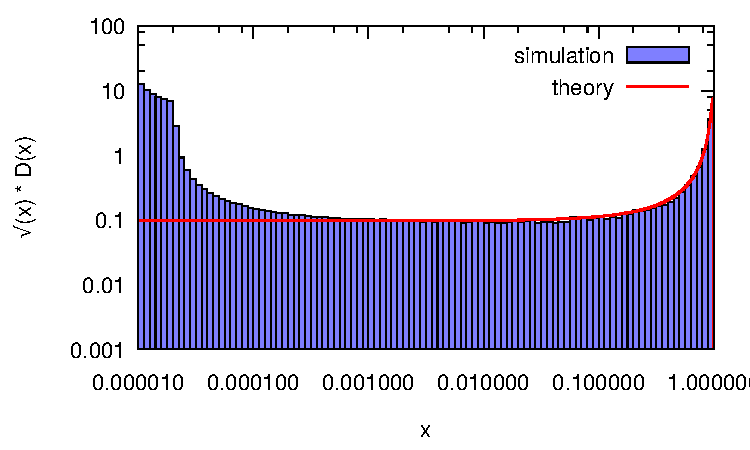
\includegraphics[width=0.65\linewidth]{Dpileup.pdf}
 % \caption{Example of pileup effect in a plot of$\sqrt{x}D(x)$ at cutoff $10^{-5}$. $\tau=0.1$.}\label{fig:D-5}
%\end{figure}



%Results go here, will probably take up 4-5 pages. (Research project took 4.)
%Btw, what is the standard for mentioning other interns? Since this is a collaborative effort Paul's name should go somewhere...


\begin{figure}
\centering
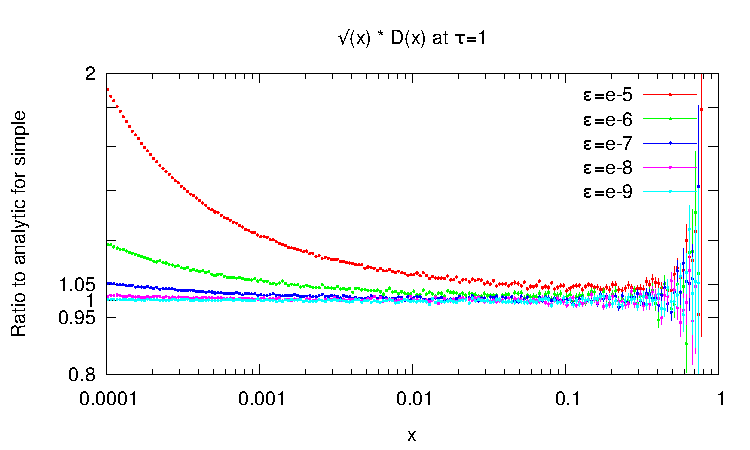
\includegraphics[width=0.9\linewidth]{convergence.pdf}
\caption{Convergence for the one point function using the simplified kernel. The ratio is taken between the numerical results, for different cutoffs $\epsilon$, and the analytic result as given by equation \eqref{Mellin}. Plotted as points with error bars.}\label{convergence}
\end{figure}

As a first step we must establish what cutoff $\epsilon$ we need to take in order to trust our values above a given $x_{min}$, which we here take to be $10^{-4}$. For the simple kernel we can compare the numerical values to the known analytic results, while for the full kernel we do not have the benefit of knowing the exact solution and must instead rely on comparing the results for higher cutoffs to the results from lowest cutoff considered. This analysis can be done for different times $\tau$ for both the one point and the two point function. A representative example is given in figure \ref{convergence}. Here we compare the numerical values of the one point function using the simple kernel to the known analytic results down to $x_{min}=10^{-4}$ for various values of $\epsilon$ ranging from $10^{-5}$ to $10^{-9}$. As we can see, taking the cutoff to $\epsilon=10^{-9}$ and considering only values above $x_{min}=10^{-4}$ will leave us with a relative error at small $x$ around one percent. Similar results can be found from testing the full kernel. 

 %In figure \ref{convergence} we compare the numerical values to the known analytic results down to $x=10^{-4}$ for various values of $\epsilon$ ranging from $10^{-5}$ to $10^{-9}$. As we can see, taking the cutoff to $\epsilon=10^{-9}$ and considering only values above $x=10^{-4}$ will leave us with a relative error at small $x$ around one percent. For the full kernel we do not have the benefit of knowing the exact solution, instead we take the ratios between the values for $\epsilon>10^{-9}$ and $\epsilon=10^{-9}$. This way we can see the convergence of the curves. Figure \ref{convergence_full} shows these ratios, and we can see that the curves show a similar convergence as for the simple kernel and that the ratio between $\epsilon=10^{-8}$ and $\epsilon=10^{-9}$ is again around one percent away from the ratio 1.



Altogether, we conclude that $\epsilon=10^{-9}$ gives sufficiently trustworthy results to continue our analysis.  The gluon spectrum is plotted for this cutoff in figure \ref{Dtimes} for $\tau=0.1,\,0.5$ and $1$. For this plot we use the full vector generated for each event and traverse it to find the gluons that were present at the relevant times. For the simplified kernel, we see that the one point spectrum matches the analytical result well, while for the  full kernel the spectrum looks slightly different. More precisely for the full kernel we see that the branching is less efficient, which is reasonable since the numerator in the splitting kernel is smaller. This is especially visible for the larger times, where we see that less energy has been lost from the spectrum. For the smaller times we see that more energy remains with the leading particle corresponding to the rightmost peak.

In order to estimate the numerical accuracy, the ratio between the numerical and results for the simplified kernel is plotted for each time, with error bars for the numerical values. This is shown in the lower part of figure \ref{Dtimes}. At large $x$ the relative error is large due to the small sample size, especially at $\tau=1$ when there is a large depletion at $x \sim 1$. The ratio of 1 is still within our statistical uncertainties. At small $x$ we see a systematic overestimation of the numerical values, here the error bars do not include the ratio 1 and so we can conclude that we have a bias. This bias also present in figure \ref{convergence}, and therefore originates at least in part from the effect of a nonzero cutoff.


In figure \ref{D2times} we show the same plot for the two point function, considering only the case $x=x'$. Here the numerical fluctuations are larger, suggesting that more iterations would be needed to get within the same statistical accuracy as for the one point function. Apart from this the behaviour is similar, again showing the effect of the full splitting kernel leading to a less efficient branching.

Overall, we can conclude that our simulation reproduces the known results for the simple kernel, and that our results give a first glimpse of the corrections to these results obtained by considering the full kernel instead. 




%\begin{figure}
%\centering
%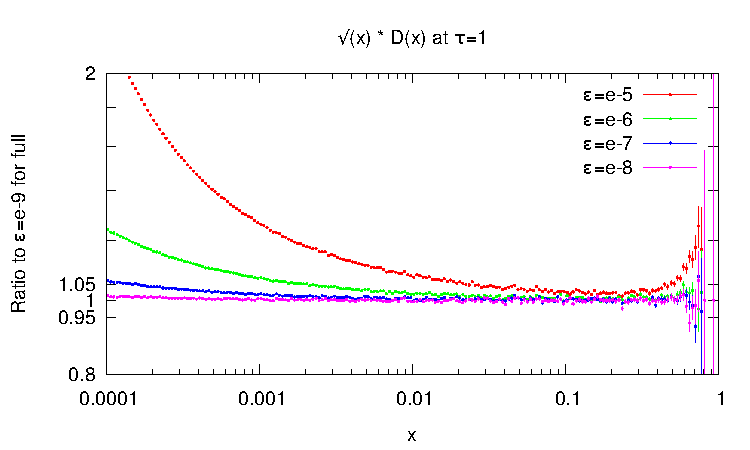
\includegraphics[width=0.8\linewidth]{convergence_full.pdf}
%\caption{Convergence for full kernel, ratio taken with the result at lowest cutoff. Plotted as points with error bars}\label{convergence_full}
%\end{figure}



\begin{figure}
\centering
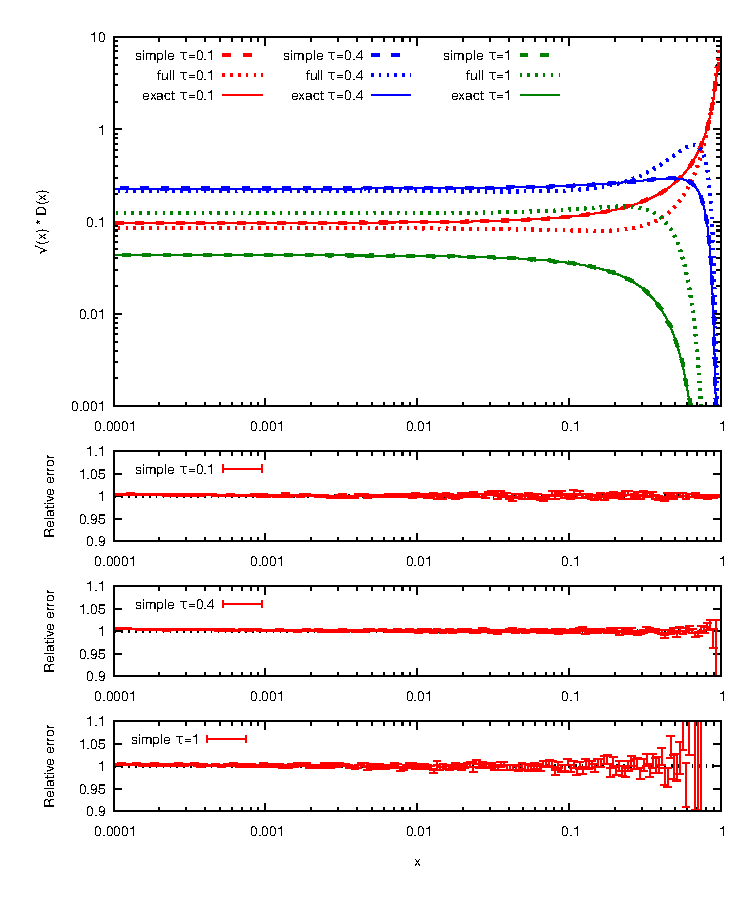
\includegraphics[width=0.9\linewidth]{times.pdf}
\vspace*{-20pt}
\caption{$\sqrt{x} D(x)$ at various times. The curves for the simple kernel overlap with the analytic solutions (as given by equation \eqref{Mellin}) for the simple kernel in the upper subplot, with the ratio between these curves shown in the lower three subplots. The curves for the full kernel depart from those of the simple kernel.}\label{Dtimes}
\end{figure}

\begin{figure}
\centering
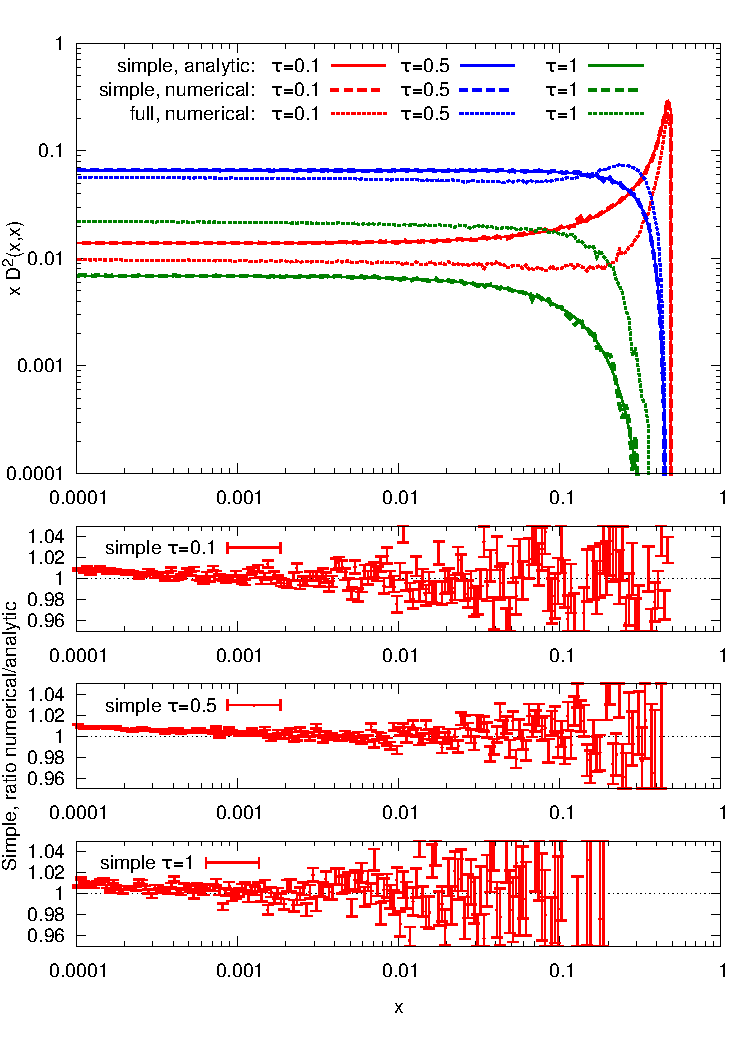
\includegraphics[width=0.9\linewidth]{D2.pdf}
\vspace*{-20pt}
\caption{$x D^{(2)}(x,x)$ at various times. The curves for the simple kernel overlap with the analytic solutions (as given by equation \eqref{D2solution}) for the simple kernel in the upper subplot, with the ratio between these curves shown in the lower three subplots. The curves for the full kernel depart from those of the simple kernel.}\label{D2times}
\end{figure}


\section{Perspective}\label{perspective}
In this report we have presented and justified a simple one-dimensional stochastic model of jet evolution in a quark gluon plasma, and described the physical implications. Notable among these are the presence of a turbulent energy cascade, which makes the energy lost from the leading particle end up at large angles, and the presence of fluctuations in the energy loss which are of the same order as the average energy loss itself. Both of these agree qualitatively with the results from the heavy ion collisions at the LHC.

We have seen that it is possible to implement a Monte Carlo simulation for the process, and that for the simple splitting kernel the numerically generated results match the values calculated analytically. This simulation can now be used to compare the simple kernel to the full one, and the results so far show that the full kernel leads to a less efficient branching. The final weeks of the internship will be spent further exploring the consequences this difference, studying physically interesting quantities such as the average energy loss and its fluctuations.

 \begin{thebibliography}{10}
 
 \bibitem{Baier:1996kr}
R.~Baier, Y.~L. Dokshitzer, A.~H. Mueller, S.~Peigne, and D.~Schiff,
  ``{Radiative Energy Loss of High Energy Quarks and Gluons in a Finite-Volume
  Quark-Gluon Plasma},''
  \href{http://dx.doi.org/10.1016/S0550-3213(96)00553-6}{{\em Nucl. Phys.}
  {\bfseries B483} (1997) 291--320},
\href{http://arxiv.org/abs/hep-ph/9607355}{{\ttfamily arXiv:hep-ph/9607355}}.
%%CITATION = HEP-PH/9607355;%%.

\bibitem{Zakharov:1997uu}
B.~G. Zakharov, ``{Radiative Energy Loss of High Energy Quarks in Finite-Size
  Nuclear Matter and Quark-Gluon Plasma},''
  \href{http://dx.doi.org/10.1134/1.567389}{{\em JETP Lett.} {\bfseries 65}
  (1997) 615--620},
\href{http://arxiv.org/abs/hep-ph/9704255}{{\ttfamily arXiv:hep-ph/9704255}}.
%%CITATION = HEP-PH/9704255;%%.

\bibitem{Blaizot:2012fh}
J.-P. Blaizot, F.~Dominguez, E.~Iancu, and Y.~Mehtar-Tani, ``{Medium-induced
  gluon branching},'' \href{http://dx.doi.org/10.1007/JHEP01(2013)143}{{\em
  JHEP} {\bfseries 1301} (2013) 143},
\href{http://arxiv.org/abs/1209.4585}{{\ttfamily arXiv:1209.4585 [hep-ph]}}.
%%CITATION = ARXIV:1209.4585;%%.


\bibitem{Blaizot:2013hx}
J.-P. Blaizot, E.~Iancu, and Y.~Mehtar-Tani, ``{Medium-induced QCD cascade:
  democratic branching and wave turbulence},''
  \href{http://dx.doi.org/10.1103/PhysRevLett.111.052001}{{\em Phys.Rev.Lett.}
  {\bfseries 111} (2013) 052001},
\href{http://arxiv.org/abs/1301.6102}{{\ttfamily arXiv:1301.6102 [hep-ph]}}.
%%CITATION = ARXIV:1301.6102;%%.

\bibitem{Aad:2010bu}
{\bfseries ATLAS} Collaboration, G.~Aad {\em et al.}, ``{Observation of a
  Centrality-Dependent Dijet Asymmetry in Lead-Lead Collisions at
  $\sqrt{s_{NN}}$= 2.76 TeV with the Atlas Detector at the LHC},''
  \href{http://dx.doi.org/10.1103/PhysRevLett.105.252303}{{\em Phys. Rev.
  Lett.} {\bfseries 105} (2010) 252303},
\href{http://arxiv.org/abs/1011.6182}{{\ttfamily arXiv:1011.6182 [hep-ex]}}.
%%CITATION = 1011.6182;%%.

\bibitem{Chatrchyan:2011sx}
{\bfseries CMS} Collaboration, S.~Chatrchyan {\em et al.}, ``{Observation and
  Studies of Jet Quenching in PbPb Collisions at Nucleon-Nucleon Center-Of-Mass
  Energy = 2.76 TeV},''
  \href{http://dx.doi.org/10.1103/PhysRevC.84.024906}{{\em Phys. Rev.}
  {\bfseries C84} (2011) 024906},
\href{http://arxiv.org/abs/1102.1957}{{\ttfamily arXiv:1102.1957 [nucl-ex]}}.
%%CITATION = 1102.1957;%%.




\bibitem{Pythia}
  T.~Sjostrand {\it et al.},
  ``{High-energy-physics event generation with PYTHIA 6.1}'',
  {\it Comput. Phys. Commun.}  {\bf 135} (2001) 238 
  %[\hepph{0010017}];
  %%CITATION = HEP-PH 0010017;%%
  T.~Sjostrand, S.~Mrenna and P.~Z.~Skands,
  ``{A Brief Introduction to PYTHIA 8.1}'',
  {\it Comput. Phys. Commun.}  {\bf 178} (2008) 852
  %[\arXiv{0710.3820} [hep-ph]].
  %%CITATION = ARXIV:0710.3820;%%

\bibitem{Herwig}
  G.~Corcella, I.~G.~Knowles, G.~Marchesini, S.~Moretti, K.~Odagiri, P.~Richardson, M.~H.~Seymour and B.~R.~Webber,
  ``HERWIG 6.5: an event generator for Hadron Emission Reactions With Interfering Gluons (including supersymmetric processes)'' {\it JHEP} {\bf 0101} (2001) 010 %[\hepph{0011363}];
  %%CITATION = doi:10.1088/1126-6708/2001/01/010;%%
  M.~Bahr {\it et al.},
  ``Herwig++ Physics and Manual,''
  {\it Eur.\ Phys.\ J.\ }{\bf C58} (2008) 639
%  [\arXiv{0803.0883} [hep-ph]]




\bibitem{SmallR}
  M.~Dasgupta, F.~Dreyer, G.~P.~Salam and G.~Soyez, ``Small-radius jets to all orders in QCD''
  {\it JHEP} {\bf 1504} (2015) 039,
  \href{https://arxiv.org/abs/1411.5182}{{\ttfamily arXiv:1411.5182 [hep-ph]}}
  %[arXiv:1411.5182 [hep-ph]].
  %%CITATION = doi:10.1007/JHEP04(2015)039;%%



\bibitem{Zapp:2012ak}
K.~C. Zapp, F.~Krauss, and U.~A. Wiedemann, ``{A perturbative framework for jet
  quenching},'' \href{http://dx.doi.org/10.1007/JHEP03(2013)080}{{\em JHEP}
  {\bfseries 03} (2013) 080},
\href{http://arxiv.org/abs/1212.1599}{{\ttfamily arXiv:1212.1599 [hep-ph]}}.
%%CITATION = ARXIV:1212.1599;%%.


  \bibitem{Schenke:2009gb}
B.~Schenke, C.~Gale, and S.~Jeon, ``{Martini: an Event Generator for
  Relativistic Heavy-Ion Collisions},''
  \href{http://dx.doi.org/10.1103/PhysRevC.80.054913}{{\em Phys. Rev.}
  {\bfseries C80} (2009) 054913},
\href{http://arxiv.org/abs/0909.2037}{{\ttfamily arXiv:0909.2037 [hep-ph]}}.
%%CITATION = 0909.2037;%%.


\bibitem{peskin}
M. E. Peskin and D. V. Shroeder, ``An Introduction to Quantum Field Theory,'' \emph{Westview Press} (1995).

 	
\bibitem{Debye}
J. P. Blaizot and E. Iancu, ``The Quark-Gluon Plasma: Collective Dynamics and Hard Thermal Loops,''
{\em Phys.Rept.} {\bf 359} (2002) 355-528,
\href{https://arxiv.org/abs/hep-ph/0101103}{{\ttfamily arXiv:0101103 [hep-ph]}}.
  
 	
\bibitem{Review}
Y. Mehtar-Tani, J. G. Milhano and K. Tywoniuk, ``Jet physics in heavy-ion collisions,''
{\em Int. J. of Mod. Phys. A} {\bf 28} (2013) 1340013,
\href{https://arxiv.org/abs/1302.2579}{{\ttfamily arXiv:1302.2579 [hep-ph]}}.
  
  



\bibitem{probabilistic}
J. P. Blaizot, F. Dominguez, E. Iancu and Y. Mehtar-Tani, ``Probabilistic picture for medium-induced jet evolution,'' {\em JHEP} {\bf 06} (2014) 075,
 \href{http://arxiv.org/abs/1311.5823}{{\ttfamily arXiv:1311.5823 [hep-ph]}}.
 	


\bibitem{FisterIancu}
 E. Iancu and L. Fister, ``Medium-induced jet evolution: wave turbulence and energy loss,''{\em JHEP} {\bf 1503} (2015) 082,
 \href{http://arxiv.org/abs/1409.2010}{{\ttfamily arXiv:1409.2010 [hep-ph]}}.






\bibitem{Escobedo:2016jbm} 
  M.~A.~Escobedo and E.~Iancu,
  ``Event-by-event fluctuations in the medium-induced jet evolution,''
  {\em JHEP} {\bf 1605}  (2016) 008,
  \href{http://arxiv.org/abs/1601.03629}{{\ttfamily  arXiv:1601.03629 [hep-ph]}}.
  



\bibitem{KNO}
M. A. Escobedo and E. Iancu, ``Multi-particle correlations and KNO scaling in the medium-induced jet evolution,''
{\em JHEP} {\bf 12} (2016) 104,
\href{https://arxiv.org/abs/1609.06104}{{\ttfamily arXiv:1609.06104 [hep-ph]}}.
 	
\end{thebibliography}
\newpage
\appendix




\section{Finding the Green's function}\label{Greendetails}
In this appendix we show the details of solving equation \eqref{Greenfunction} with the initial condition $G(x,x_0,\tau=0)=\delta(x-x_0)$. We note that the solution to equation \eqref{Devo}, given by equation \eqref{Mellin}, is a function with the correct behaviour \emph{if} we have $x_0=1$. Indeed, since the structure of equations \eqref{D2evo} and \eqref{Devo} is the same, we have
\begin{equation}
L D(x,\tau)=0,
\end{equation}
with $D(x,0)=\delta(x-1)$.


We thus want to modify this solution to allow for any value of $x_0$. To make this explicit, we can go back to our physical variables. Let us write
\begin{equation}
G(x,x_0,\tau)=g(\omega, \omega_0,t),
\end{equation}
with $x \equiv w/E$, $x_0 \equiv \omega_0/E$ and $\tau \equiv t/\Delta t_{br}(E)$, $\omega < \omega_0 <E$. In these variables our goal is to replace $E$ by $x_0$ in the one point function $D$. However, for our initial condition we want
\begin{equation}
G(x,x_0,0)=g(\omega,\omega_0,0)=\delta(x-x_0)=\delta \left( \frac{\omega}{E} - \frac{\omega_0}{E}\right)=E\delta(\omega-\omega_0).
\end{equation}
We can see that it is not enough to take $D(x,0)$ and naively make a substitution $E\rightarrow \omega$, since this would give the initial condition
\begin{equation}
D(x,0)=\delta\left(\frac{\omega}{E}-1\right)=E\delta(\omega-E)\rightarrow \omega_0 \delta(\omega-\omega_0).
\end{equation}
Clearly we will need to compensate by a factor $E/\omega_0$, which in our rescaled variables reads $1/x_0$.

With this compensation out of the way we should consider the dependence within $D$ of $E$, and hence of $x_0$:
\begin{equation}
g(\omega,E,t)=D(x,\tau)=D\left( \frac{\omega}{E},\frac{t}{\Delta t_{br}(E)}\right)=\tilde{D} \left( \frac{\omega}{E},\frac{t}{\sqrt{E}}\right).
\end{equation}
In the redefined $\tilde{D}$ the dependence on $E$ has been made explicit. We now let $E\rightarrow \omega_0$ and obtain
\begin{equation}
\tilde{D}\left( \frac{\omega}{\omega_0},\frac{t}{\sqrt{\omega_0}}\right)=\tilde{D}\left( \frac{\omega}{\omega_0},\frac{t}{\sqrt{x_0 E}}\right)=D\left( \frac{x}{x_0},\frac{\tau}{\sqrt{x_0}}\right).
\end{equation}
Taking these considerations together we obtain our result
\begin{equation}
G(x,x_0,\tau) = \frac{1}{x_0} D\left(\frac{x}{x_0},\frac{\tau}{\sqrt{x_0}}\right).
\end{equation}

\newpage
\section{Code}\label{code}
This appendix shows the code for the recursive branching function, {\tt \char`_branch}, which is a member function of a class {\tt GeneratorInMedium} that is used whenever we want to generate an event. As a convention, all variables and functions preceded by an underscore are private members of {\tt GeneratorInMedium}. 
The simulation is written in C++ and makes use of the GNU Scientific Library\footnote{\url{https://www.gnu.org/software/gsl/}} for generating (pseudo-)random numbers.

\begin{lstlisting}
/// Branches the last particle in _particles
void GeneratorInMedium::_branch(){
  unsigned int parent=_particles.size()-1;

  double x=_particles[parent].x();///< Relies on pushing back child before branching
  if(x<_xmin){
    return;///< We have reached the bottom of the recursion => we have one particle.
  }
  /// SplittingTime, randomly generated
  generate_branching(x);
  double splitting_time=_t;
  double z=_z;

  double time_left=_end_time - _particles[parent].start_time();
  if(time_left < splitting_time){
    return;///< We have reached the bottom of the recursion => we have one particle.
  }
  /// No "if" triggered =>we have time enough for another split and x is large enough
  double current_time=_particles[parent].start_time() + splitting_time;
  _particles[parent].set_end_time(current_time);
  /// To add to the vector storing the event
  Particle child1(parent,current_time,z*x), child2(parent,current_time,(1-z)*x);

  /// Branching into two
  /// First child:
  _particles.push_back(child1);
  _particles[parent].set_child1(_particles.size()-1);
  _branch();
  ///Second child:
  _particles.push_back(child2);
  _particles[parent].set_child2(_particles.size()-1);
  _branch();
}
\end{lstlisting}




\end{document}\grid
